\documentclass[11pt]{article}
\usepackage[margin=1in]{geometry}
\usepackage[T1]{fontenc}
\usepackage[utf8]{inputenc}
\usepackage{lmodern}
\usepackage{graphicx}
\usepackage{booktabs}
\usepackage{longtable}
\usepackage{float}
\usepackage{array}
\usepackage{hyperref}
\hypersetup{colorlinks=true,linkcolor=black,urlcolor=blue,citecolor=black}
\title{Tobit Regression Analysis Report}
\author{Automated Analysis Pipeline}
\date{Generated on 2026-03-22 11:32 -05}
\begin{document}
\maketitle
\begin{abstract}
This report documents the full Tobit analysis workflow for the Florida experiment dataset, including materials, data cleaning, long-format transformation, bounded-outcome modeling, statistical interpretation, assumptions, and conclusions.
\end{abstract}
\section{Introduction}
This report evaluates how empathy and social identity relate to moral judgments of negotiators in an incentivized experiment. The reporting workflow is designed to be reproducible and publication-oriented, using the same fitted models that drive the Markdown and Word outputs.
\section{Materials and Methods}
\subsection{Inputs and Materials}
Dataset: data\_final\_FLORIDA.xlsx Codebook: datacard.md Hypotheses source: hypotheses.md .
Materials. The analysis uses the workbook data\_final\_FLORIDA.xlsx, the project codebook datacard.md, and the substantive framing in hypotheses.md. The source workbook contains 63 participant rows and repeated scenario blocks for 10 stages, with two negotiator decisions and two numerical judgments per stage. Methods. The pipeline reshapes the workbook from wide participant format to long negotiator-level format, scores the Interpersonal Reactivity Index, filters the primary analysis sample using the attention checks, estimates Tobit regressions for the bounded outcome, and exports tables, figures, Markdown, Word, LaTeX, and PDF reports.
\subsection{Sample and Data Structure}
The workbook contains 63 participants, of whom 58 passed both attention checks. The primary analysis retains 58 participants and 1160 negotiator-level judgments. The Tobit hypothesis models focus on 569 harmful decisions in which a negotiator accepted the payoff-increasing but victim-harming deal.
\begin{table}[H]
\centering
\caption{Participant summary.}
\label{tab:participant_summary}
\begin{tabular}{ll}
\toprule
Metric & Value \\
\midrule
Participants in workbook & 63.000 \\
Participants passing both attention checks & 58.000 \\
Participants in primary analysis & 58.000 \\
Mean age (analysis sample) & 20.293 \\
SD age (analysis sample) & 4.877 \\
Women in analysis sample & 27.000 \\
Men in analysis sample & 31.000 \\
Humanities in analysis sample & 27.000 \\
Engineering in analysis sample & 31.000 \\
Victim-first treatment in analysis sample & 29.000 \\
Observer-first treatment in analysis sample & 29.000 \\
\bottomrule
\end{tabular}
\end{table}
\subsection{Data Cleaning and Step-by-Step Data Handling}
Data cleaning proceeded in explicit steps. Step 1: validate that all required participant-level and scenario-level columns are present in the workbook. Step 2: preserve the raw participant-level file, generate stage-specific role indicators, and derive IRI composite and subscale scores. Step 3: compute the attention-check flag and define the primary analysis sample as participants who passed both checks, had a non-missing IRI composite, and are in treatment 1 or 2. Step 4: reshape the repeated scenario variables into negotiator-level long format, yielding two judgment rows per stage per participant. Step 5: derive perpetrator alignment, victim alignment, same-group harm, and harmful-decision indicators. In this dataset, 0 participants were excluded for treatment = 0, 5 participants fail at least one attention check, and 0 participants have a missing IRI composite, leaving 58 participants in the primary sample.
\subsection{Variable Transformation and Analysis Setup}
Variable handling and transformation were kept close to the observed data structure. The dependent variable is the raw judgment score, bounded between -9 and 9, and it is modeled directly rather than transformed into a severity index. The empathy predictor is standardized as iri\_total\_z so its coefficient reflects a one-standard-deviation change in empathy. The main hypothesis models are restricted to harmful decisions where decision\_accept = 1, because the hypotheses concern condemnation of harmful conduct rather than neutral or prosocial choices. Control variables include observer role, participant faculty, sex, age, socioeconomic status, stage indicators, and negotiator-slot indicators.
\subsection{Word-Friendly Model Equations}
\begin{flushleft}
\textbf{Observed outcome definition}\\
y\_ij = -9 if y*\_ij <= -9\\
y\_ij = y*\_ij if -9 < y*\_ij < 9\\
y\_ij = 9 if y*\_ij >= 9\\[0.4em]
\textbf{Main harmful-decision model}\\
y*\_ij = beta0 + beta1*IRI\_i + beta2*OutgroupPerp\_ij + beta3*ControlPerp\_ij + beta4*VictimOutgroup\_ij + beta5*(IRI\_i*OutgroupPerp\_ij) + beta6*(IRI\_i*ControlPerp\_ij) + gamma'*X\_ij + e\_ij\\[0.4em]
\textbf{Same-group-harm model}\\
y*\_ij = alpha0 + alpha1*IRI\_i + alpha2*SameGroupHarm\_ij + alpha3*OutgroupPerp\_ij + alpha4*VictimOutgroup\_ij + delta'*X\_ij + u\_ij
\end{flushleft}
\subsection{Empathy Scale Quality}
\begin{table}[H]
\centering
\caption{Empathy scale summary.}
\label{tab:empathy_summary}
\begin{tabular}{lllllll}
\toprule
Scale & Items & Mean & SD & Min & Max & Alpha \\
\midrule
IRI total & 28 & 2.196 & 0.448 & 1.036 & 3.250 & 0.767 \\
Fantasy & 7 & 2.111 & 0.723 & 0.286 & 4.000 & 0.644 \\
Empathic concern & 8 & 2.222 & 0.485 & 1.125 & 3.125 & 0.299 \\
Perspective taking & 7 & 2.488 & 0.665 & 0.571 & 3.714 & 0.597 \\
Personal distress & 6 & 1.918 & 0.635 & 0.000 & 3.000 & 0.521 \\
\bottomrule
\end{tabular}
\end{table}
\section{Results}
\subsection{Exploratory Data Analysis}
We first explore the raw dependent variable, showing its bounded nature and the piling up at the endpoints which justifies the Tobit approach.
\begin{figure}[H]
\centering
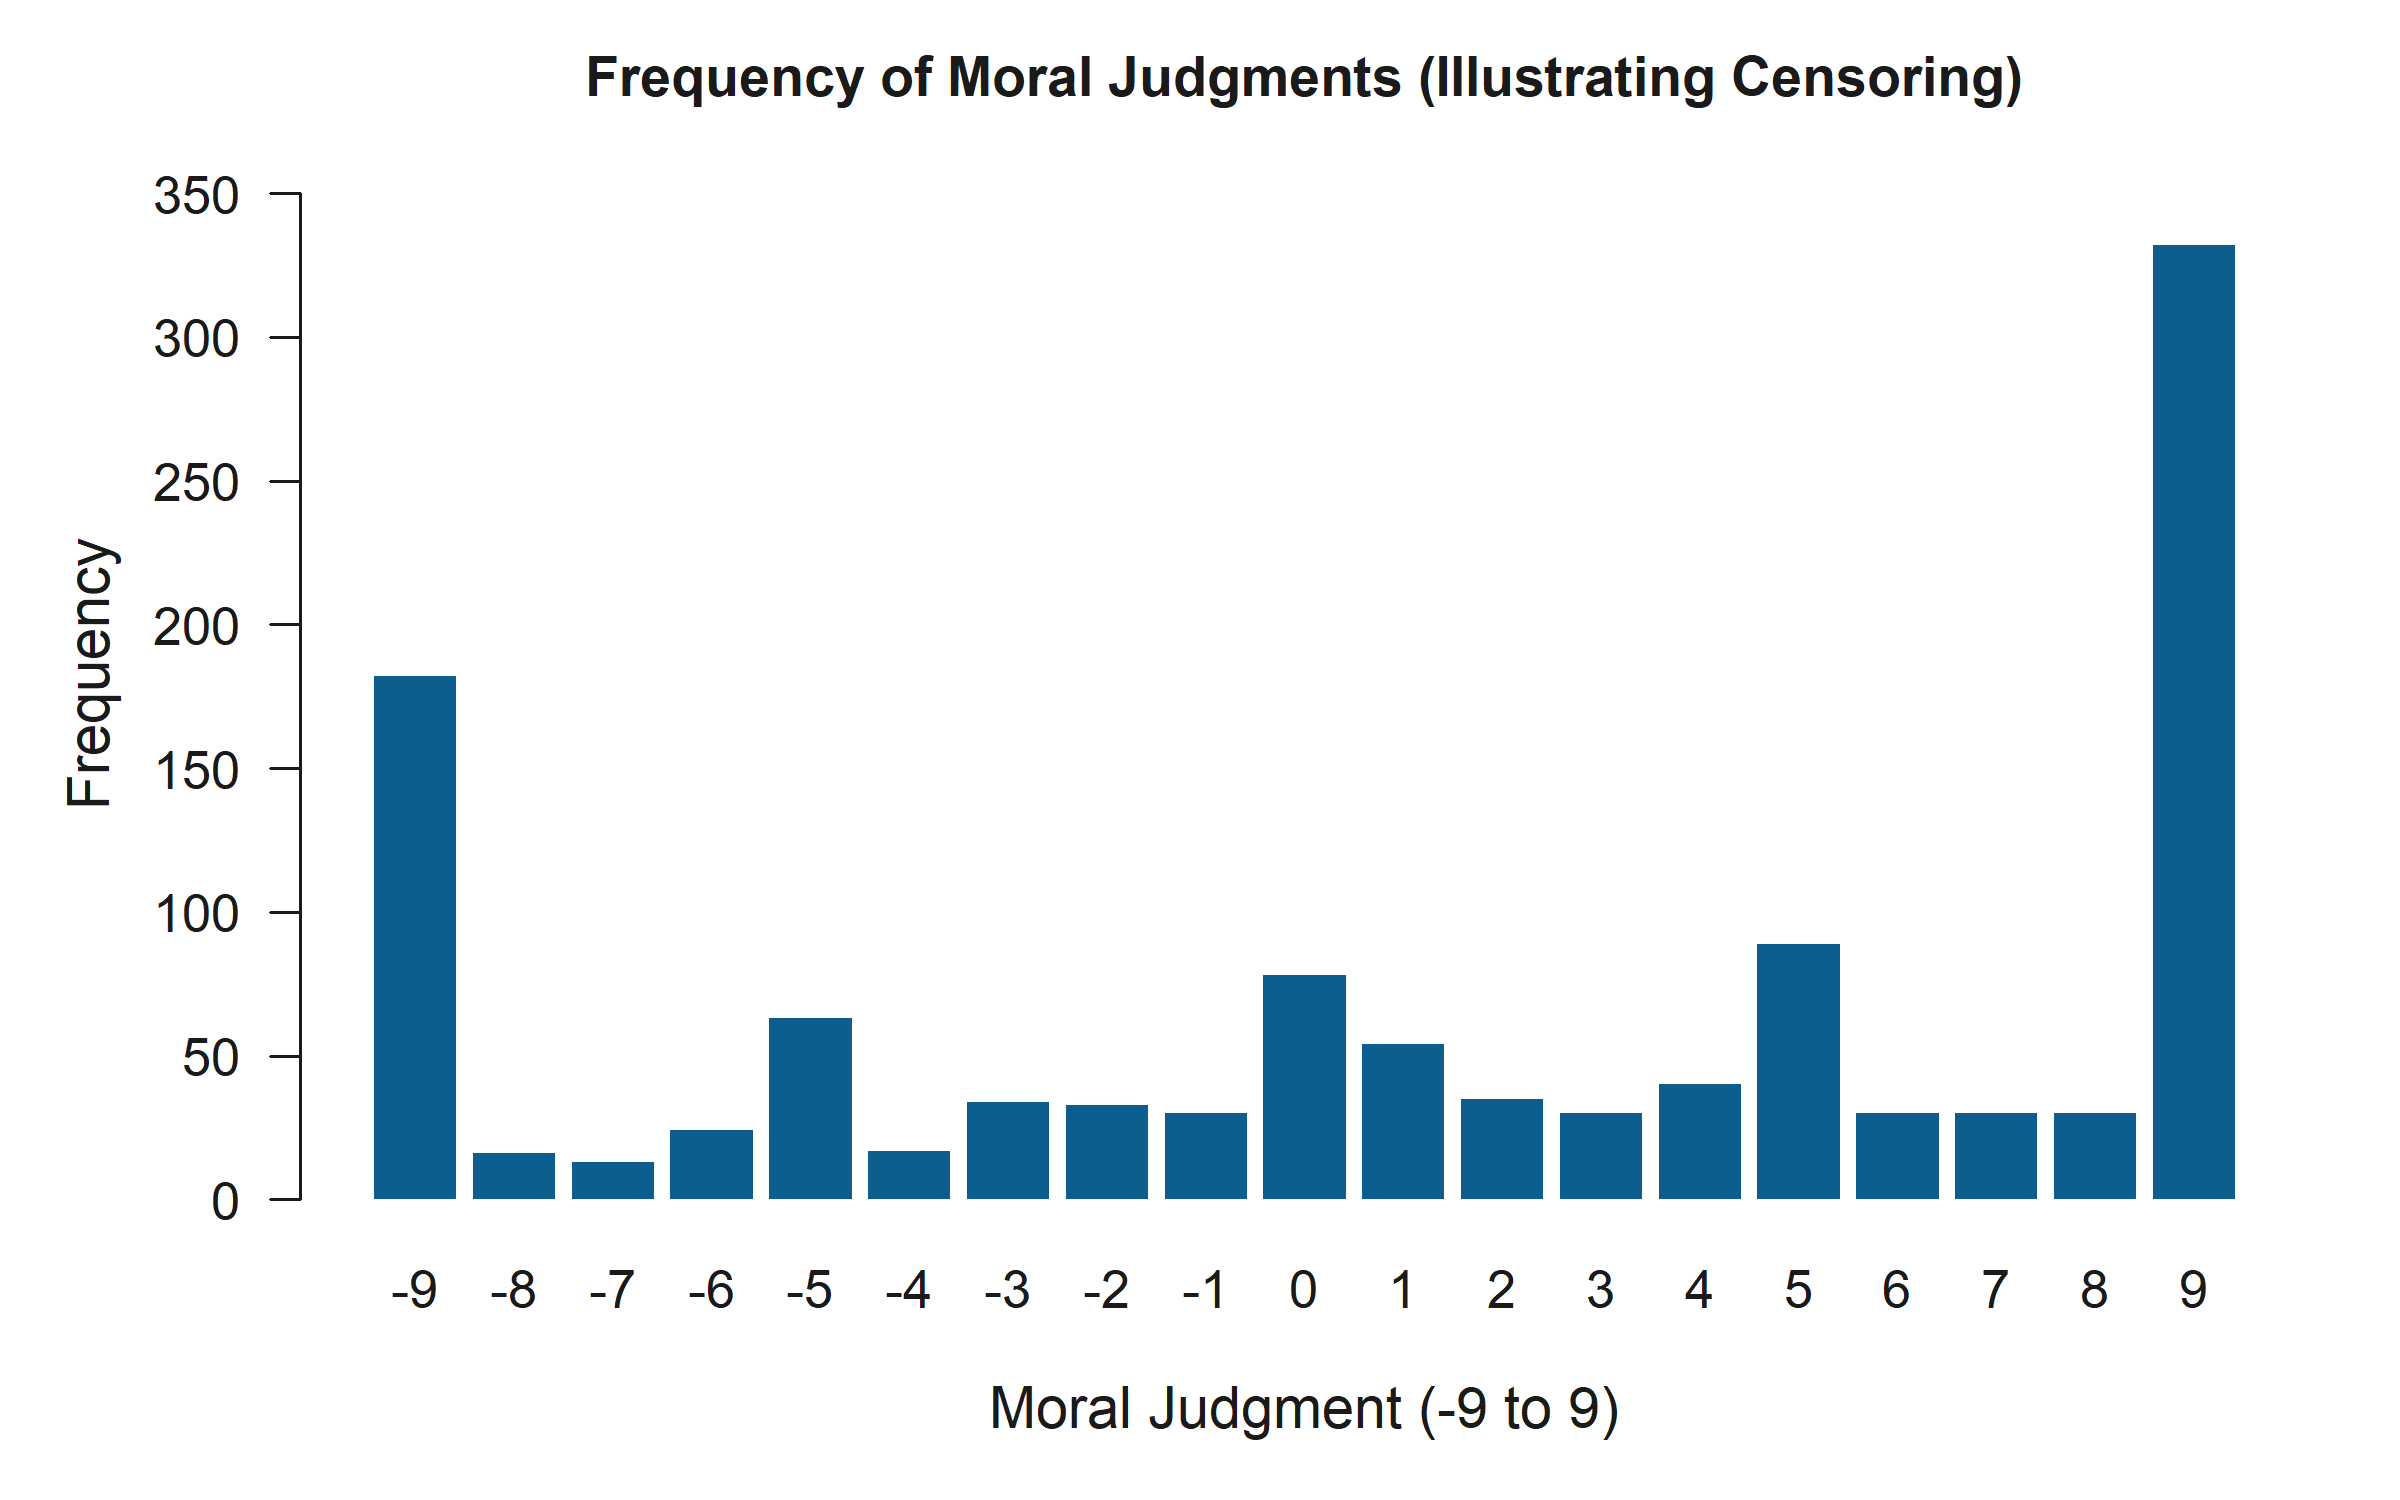
\includegraphics[width=0.92\textwidth]{../figures/figure_eda_judgement_frequency.png}
\caption{Frequency of moral judgments illustrating censoring.}
\label{fig:eda_freq}
\end{figure}
Additionally, the following table and scatterplots summarize the relationship between moral judgments and each empathy subscale.
\begin{table}[H]
\centering
\caption{Pearson correlations between judgements and empathy subscales.}
\label{tab:eda_correlations}
\begin{tabular}{lllll}
\toprule
Subscale & Pearson\_r & P\_value & CI\_low & CI\_high \\
\midrule
iri\_total & 0.008 & 0.785 & -0.050 & 0.066 \\
iri\_fs & 0.005 & 0.856 & -0.052 & 0.063 \\
iri\_ec & -0.092 & 0.002 & -0.149 & -0.034 \\
iri\_pt & 0.042 & 0.154 & -0.016 & 0.099 \\
iri\_pd & 0.061 & 0.037 & 0.004 & 0.118 \\
\bottomrule
\end{tabular}
\end{table}
\begin{figure}[H]
\centering
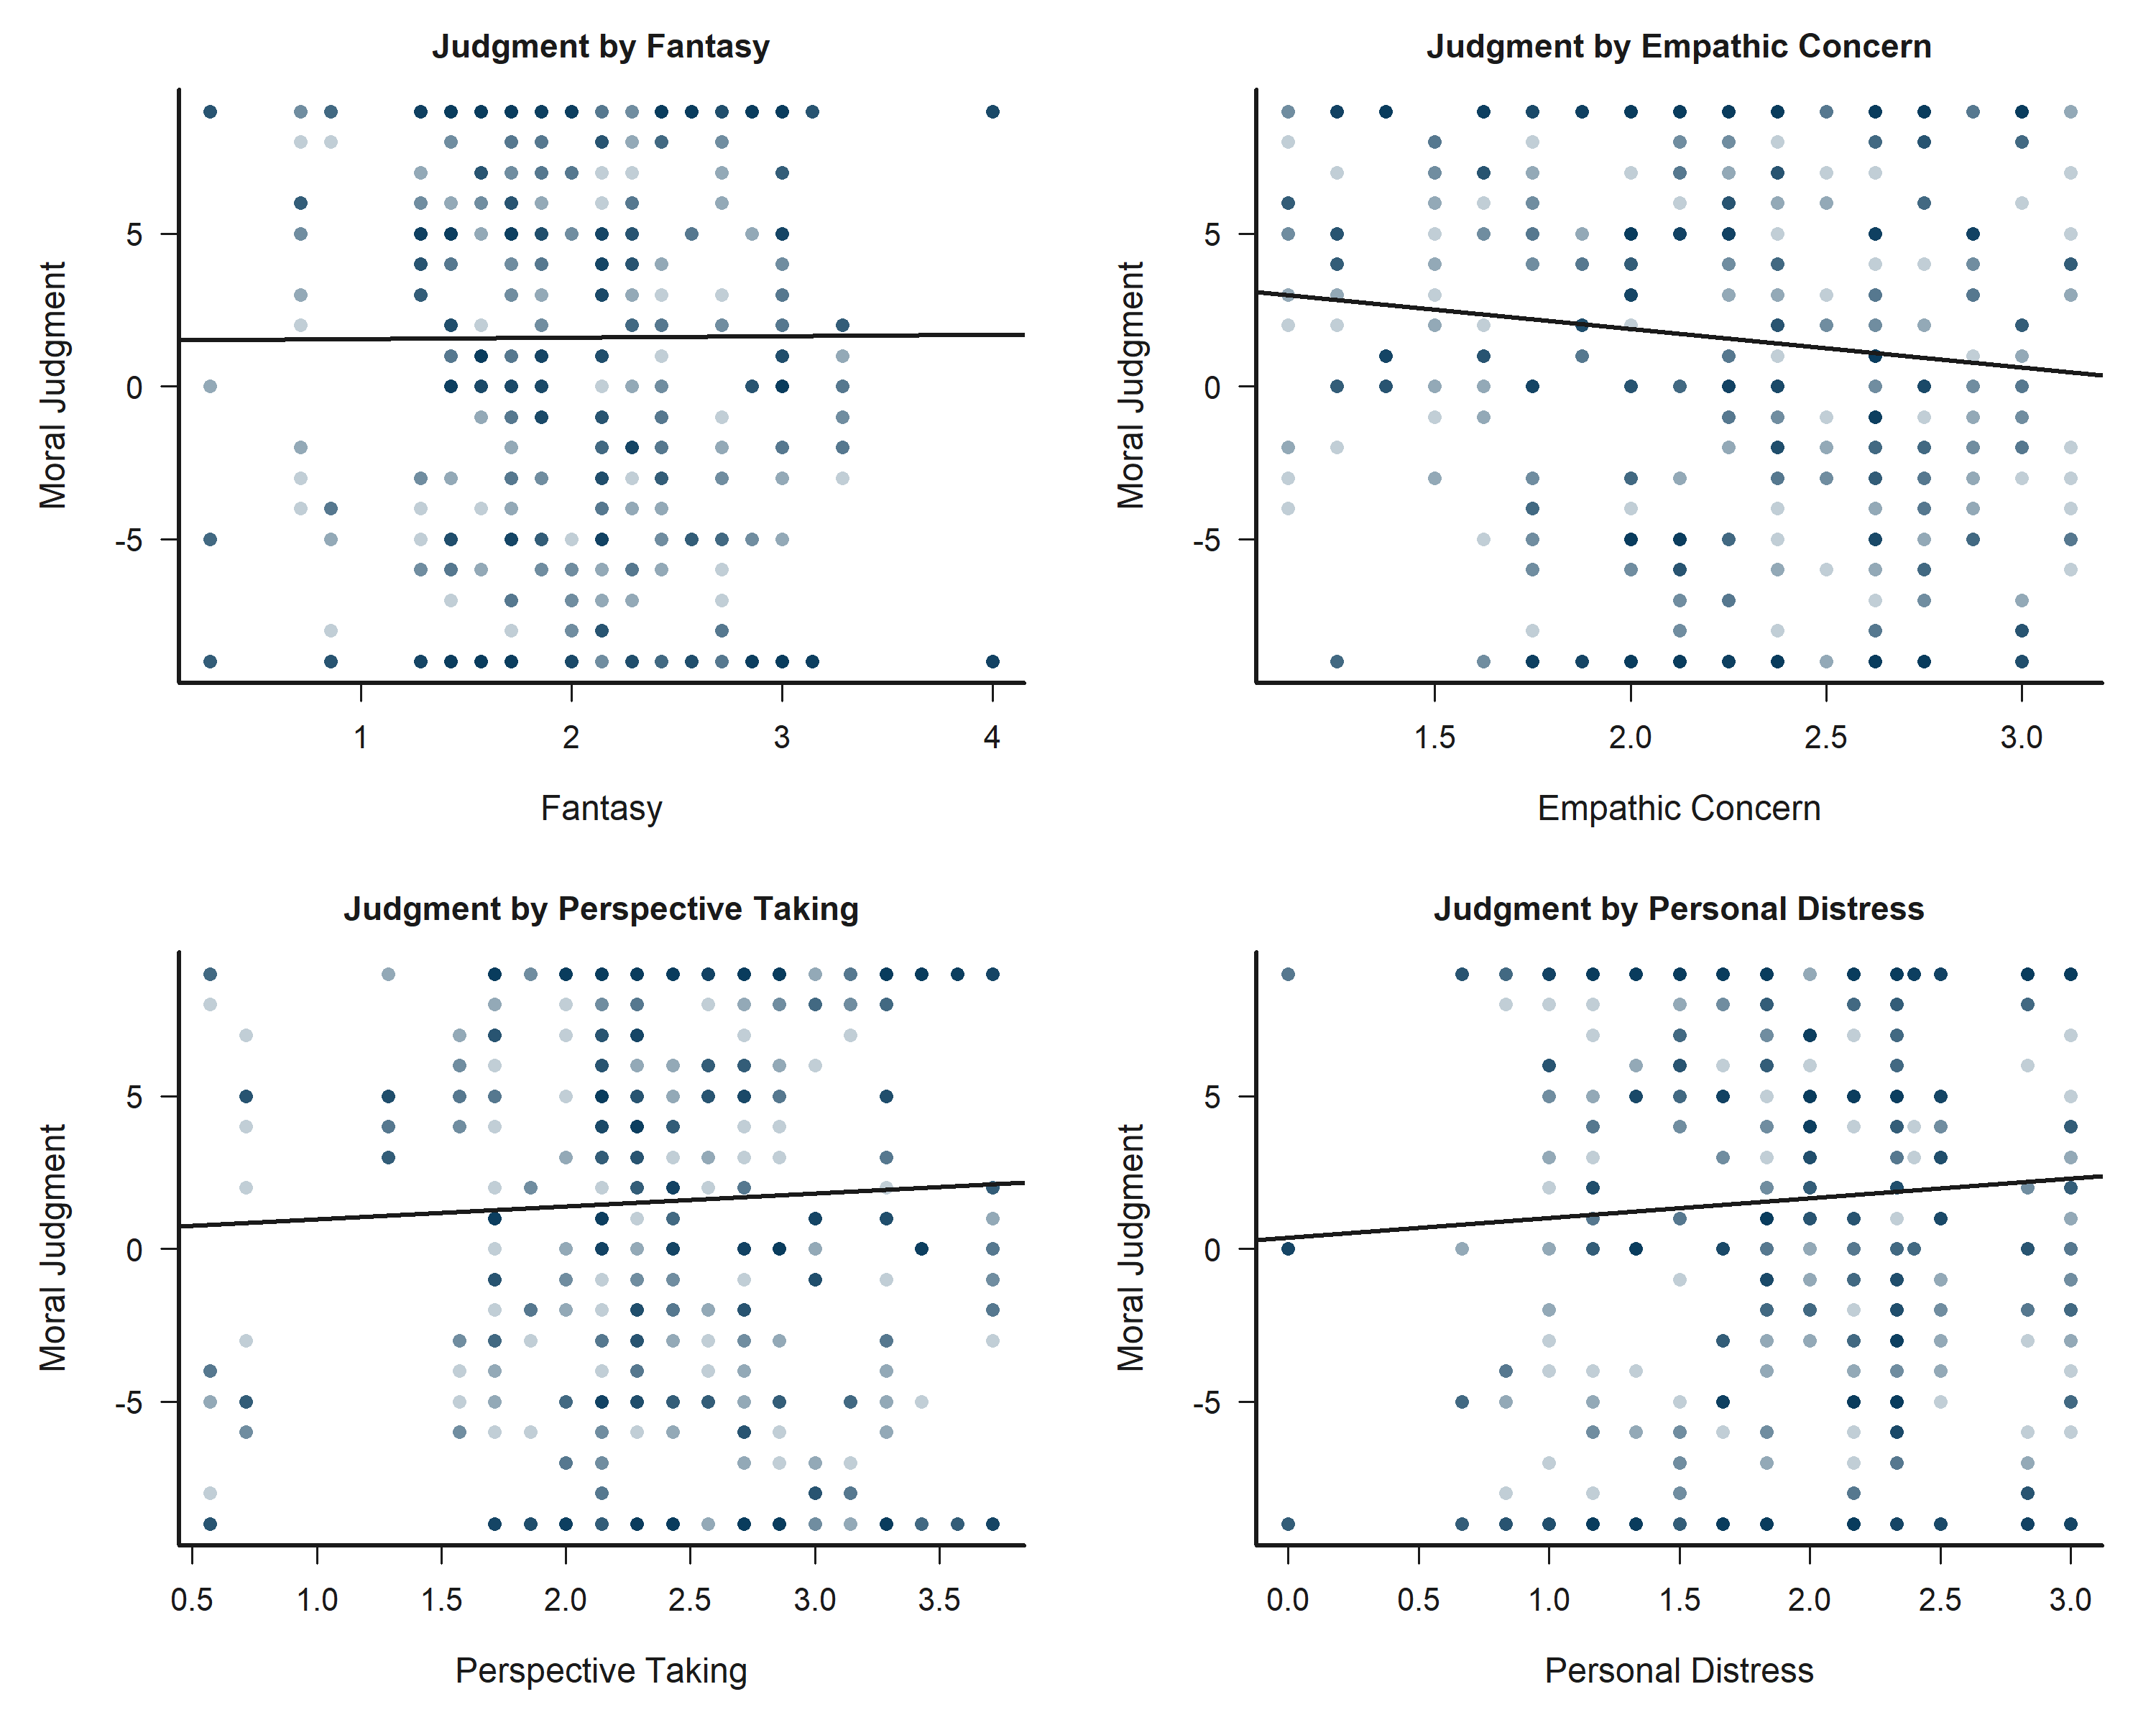
\includegraphics[width=0.92\textwidth]{../figures/figure_eda_judgement_by_iri.png}
\caption{Scatterplots of judgment by IRI subscales.}
\label{fig:eda_scatter}
\end{figure}
\subsection{Descriptive Results}
The observed Tobit outcome is the raw moral-judgment score from -9 to 9, where lower values indicate harsher condemnation. Descriptively, accepted harmful deals receive much lower ratings than rejected deals (mean judgment -3.19 versus 6.21 ). Within the harmful-decision sample, same-faculty harm averages -3.55 judgment points compared with -2.91 for cross-faculty harm. Outgroup perpetrators average -3.12 judgment points versus -3.34 for labeled ingroup perpetrators.
\begin{table}[H]
\centering
\caption{Judgment summary.}
\label{tab:judgement_summary}
\begin{tabular}{ll}
\toprule
Metric & Value \\
\midrule
Negotiator-level judgments in analysis sample & 1160.000 \\
Harmful decisions in primary model sample & 569.000 \\
Acceptance rate in analysis sample & 0.491 \\
Mean raw judgment for rejected decisions & 6.212 \\
Mean raw judgment for accepted decisions & -3.192 \\
Left-censored share at -9 in accepted sample & 0.299 \\
Right-censored share at 9 in accepted sample & 0.047 \\
\bottomrule
\end{tabular}
\end{table}
\begin{table}[H]
\centering
\caption{Harmful-decision descriptive summary by group and role.}
\label{tab:harmful_summary}
\begin{tabular}{llllllll}
\toprule
negotiator\_alignment & role & Observations & MeanJudgement & SDJudgement & SEJudgement & Lower95 & Upper95 \\
\midrule
ingroup & victim & 95 & -3.979 & 4.842 & 0.497 & -4.953 & -3.005 \\
outgroup & victim & 97 & -3.289 & 5.278 & 0.536 & -4.339 & -2.238 \\
control & victim & 104 & -3.740 & 5.593 & 0.548 & -4.815 & -2.665 \\
ingroup & observer & 92 & -2.685 & 5.056 & 0.527 & -3.718 & -1.652 \\
outgroup & observer & 80 & -2.913 & 5.406 & 0.604 & -4.097 & -1.728 \\
control & observer & 101 & -2.475 & 5.723 & 0.569 & -3.591 & -1.359 \\
\bottomrule
\end{tabular}
\end{table}
\begin{figure}[H]
\centering
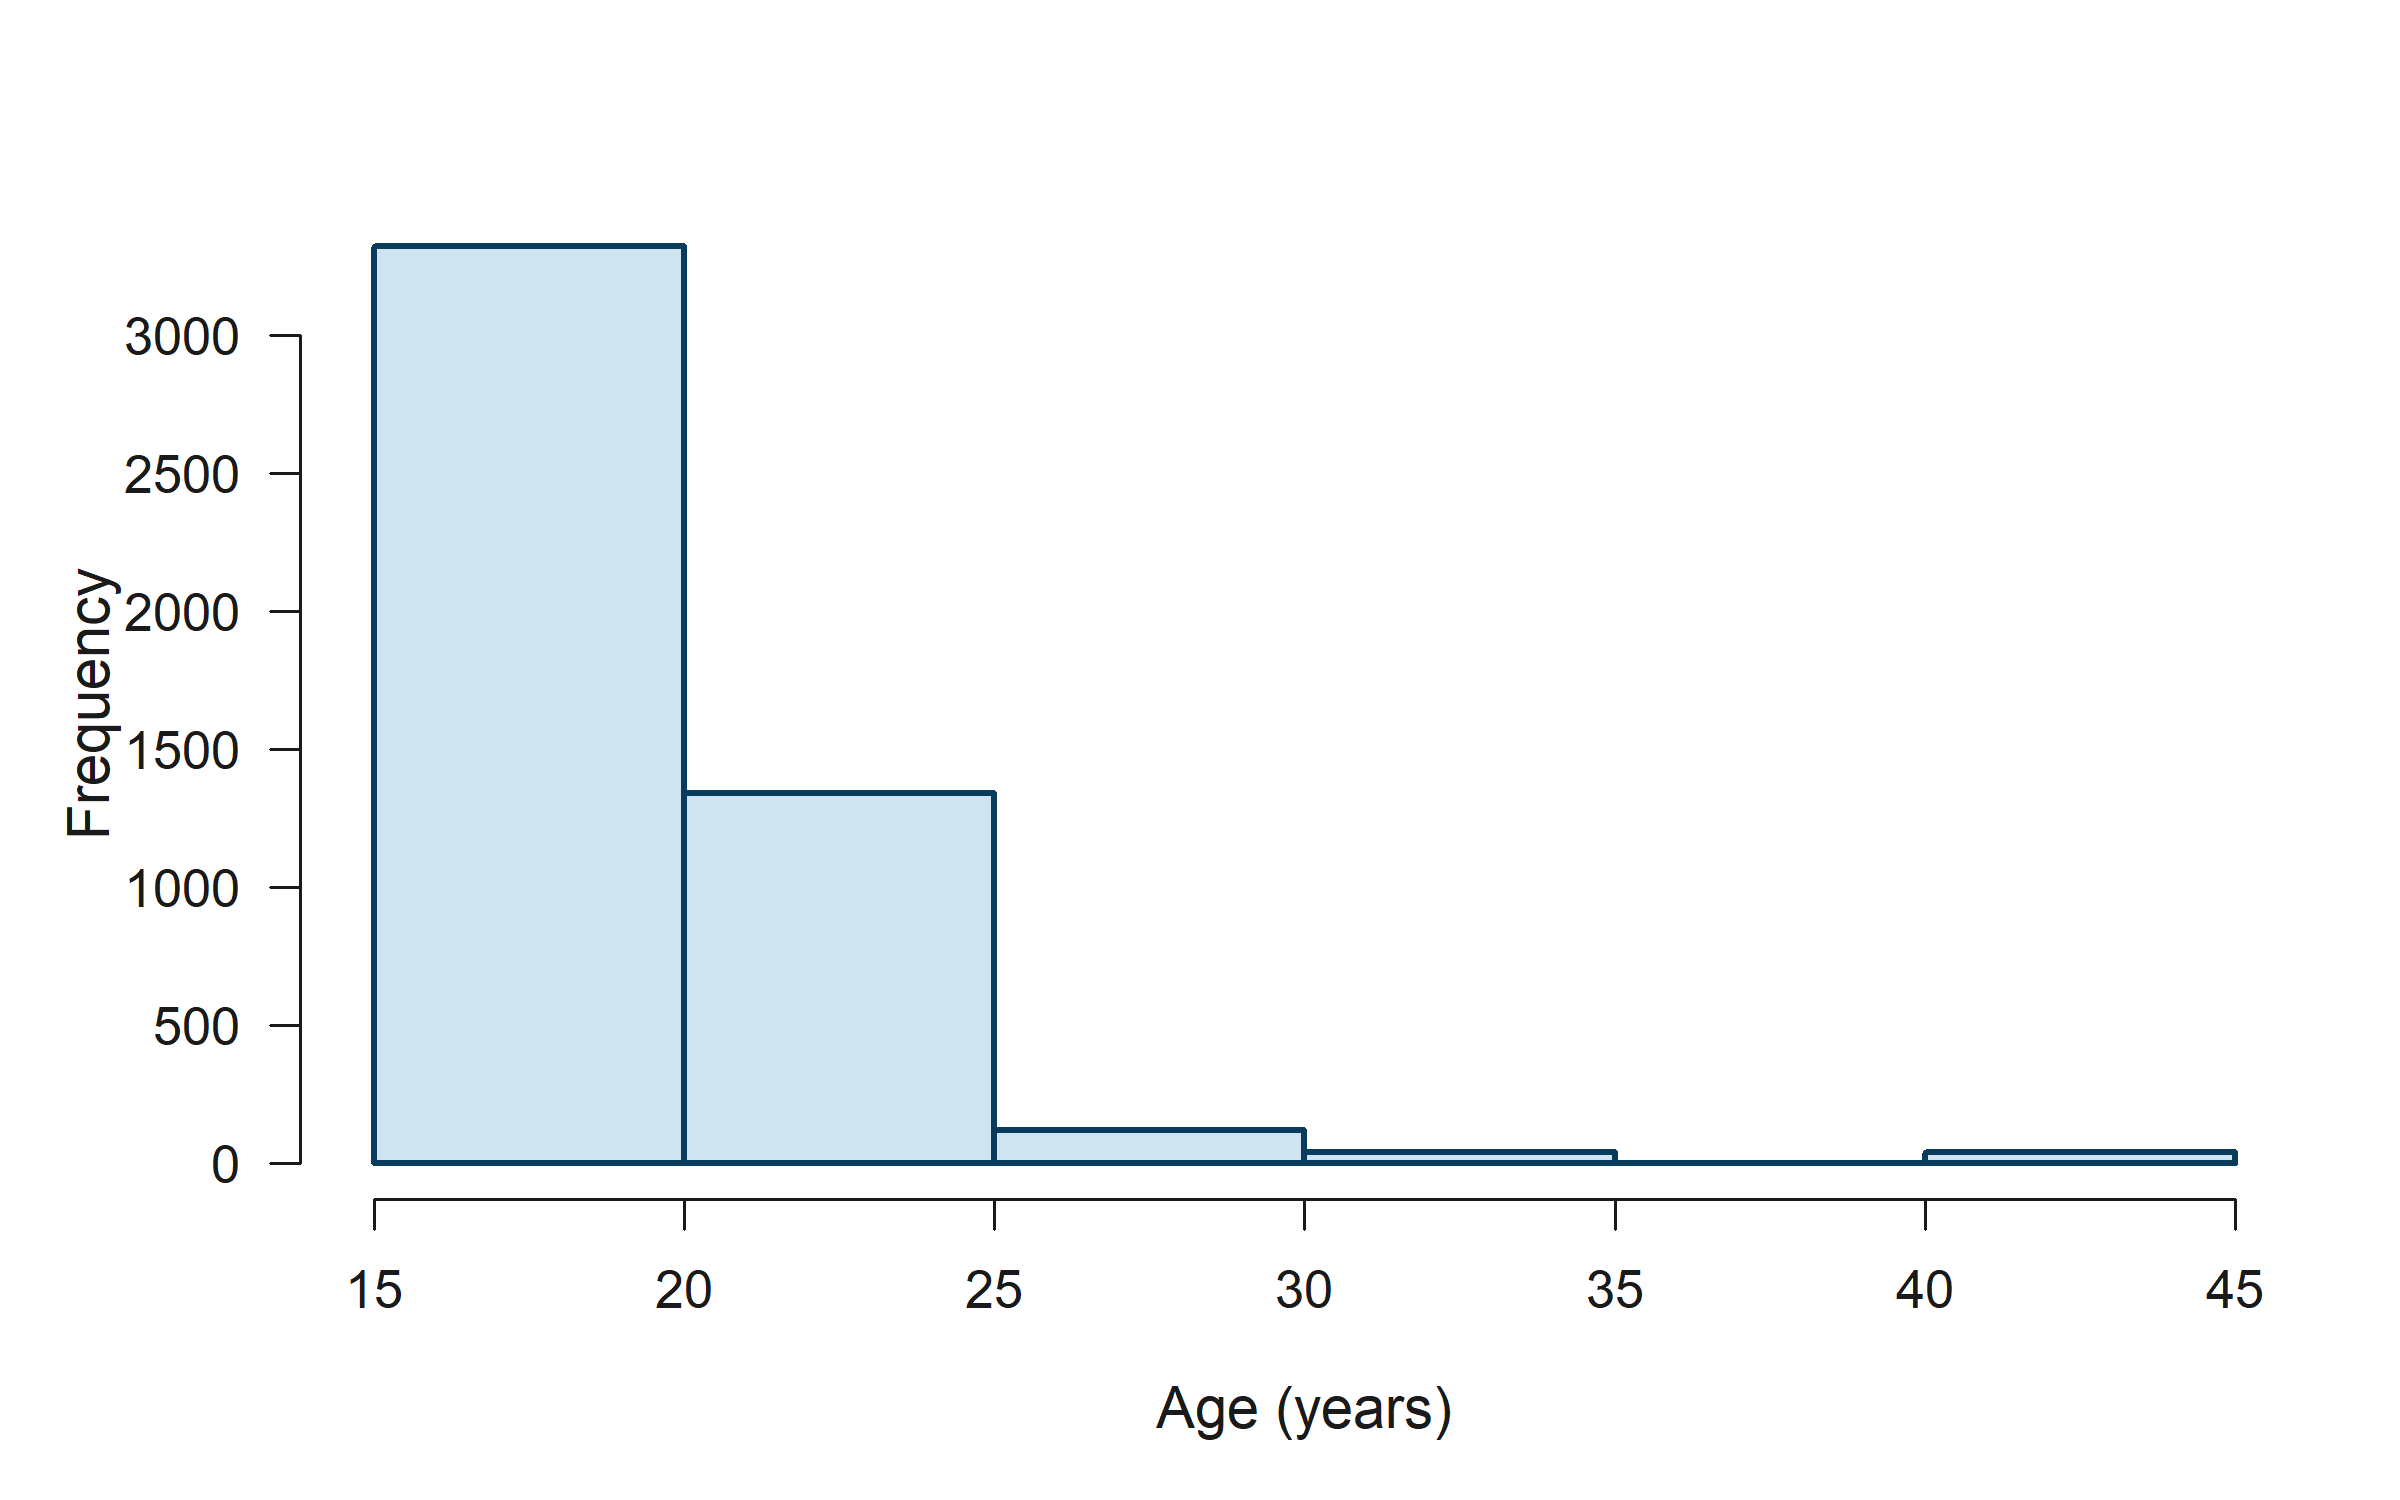
\includegraphics[width=0.92\textwidth]{../figures/figure_01_age_distribution.png}
\caption{Age distribution in the analysis sample.}
\label{fig:age}
\end{figure}
\begin{figure}[H]
\centering
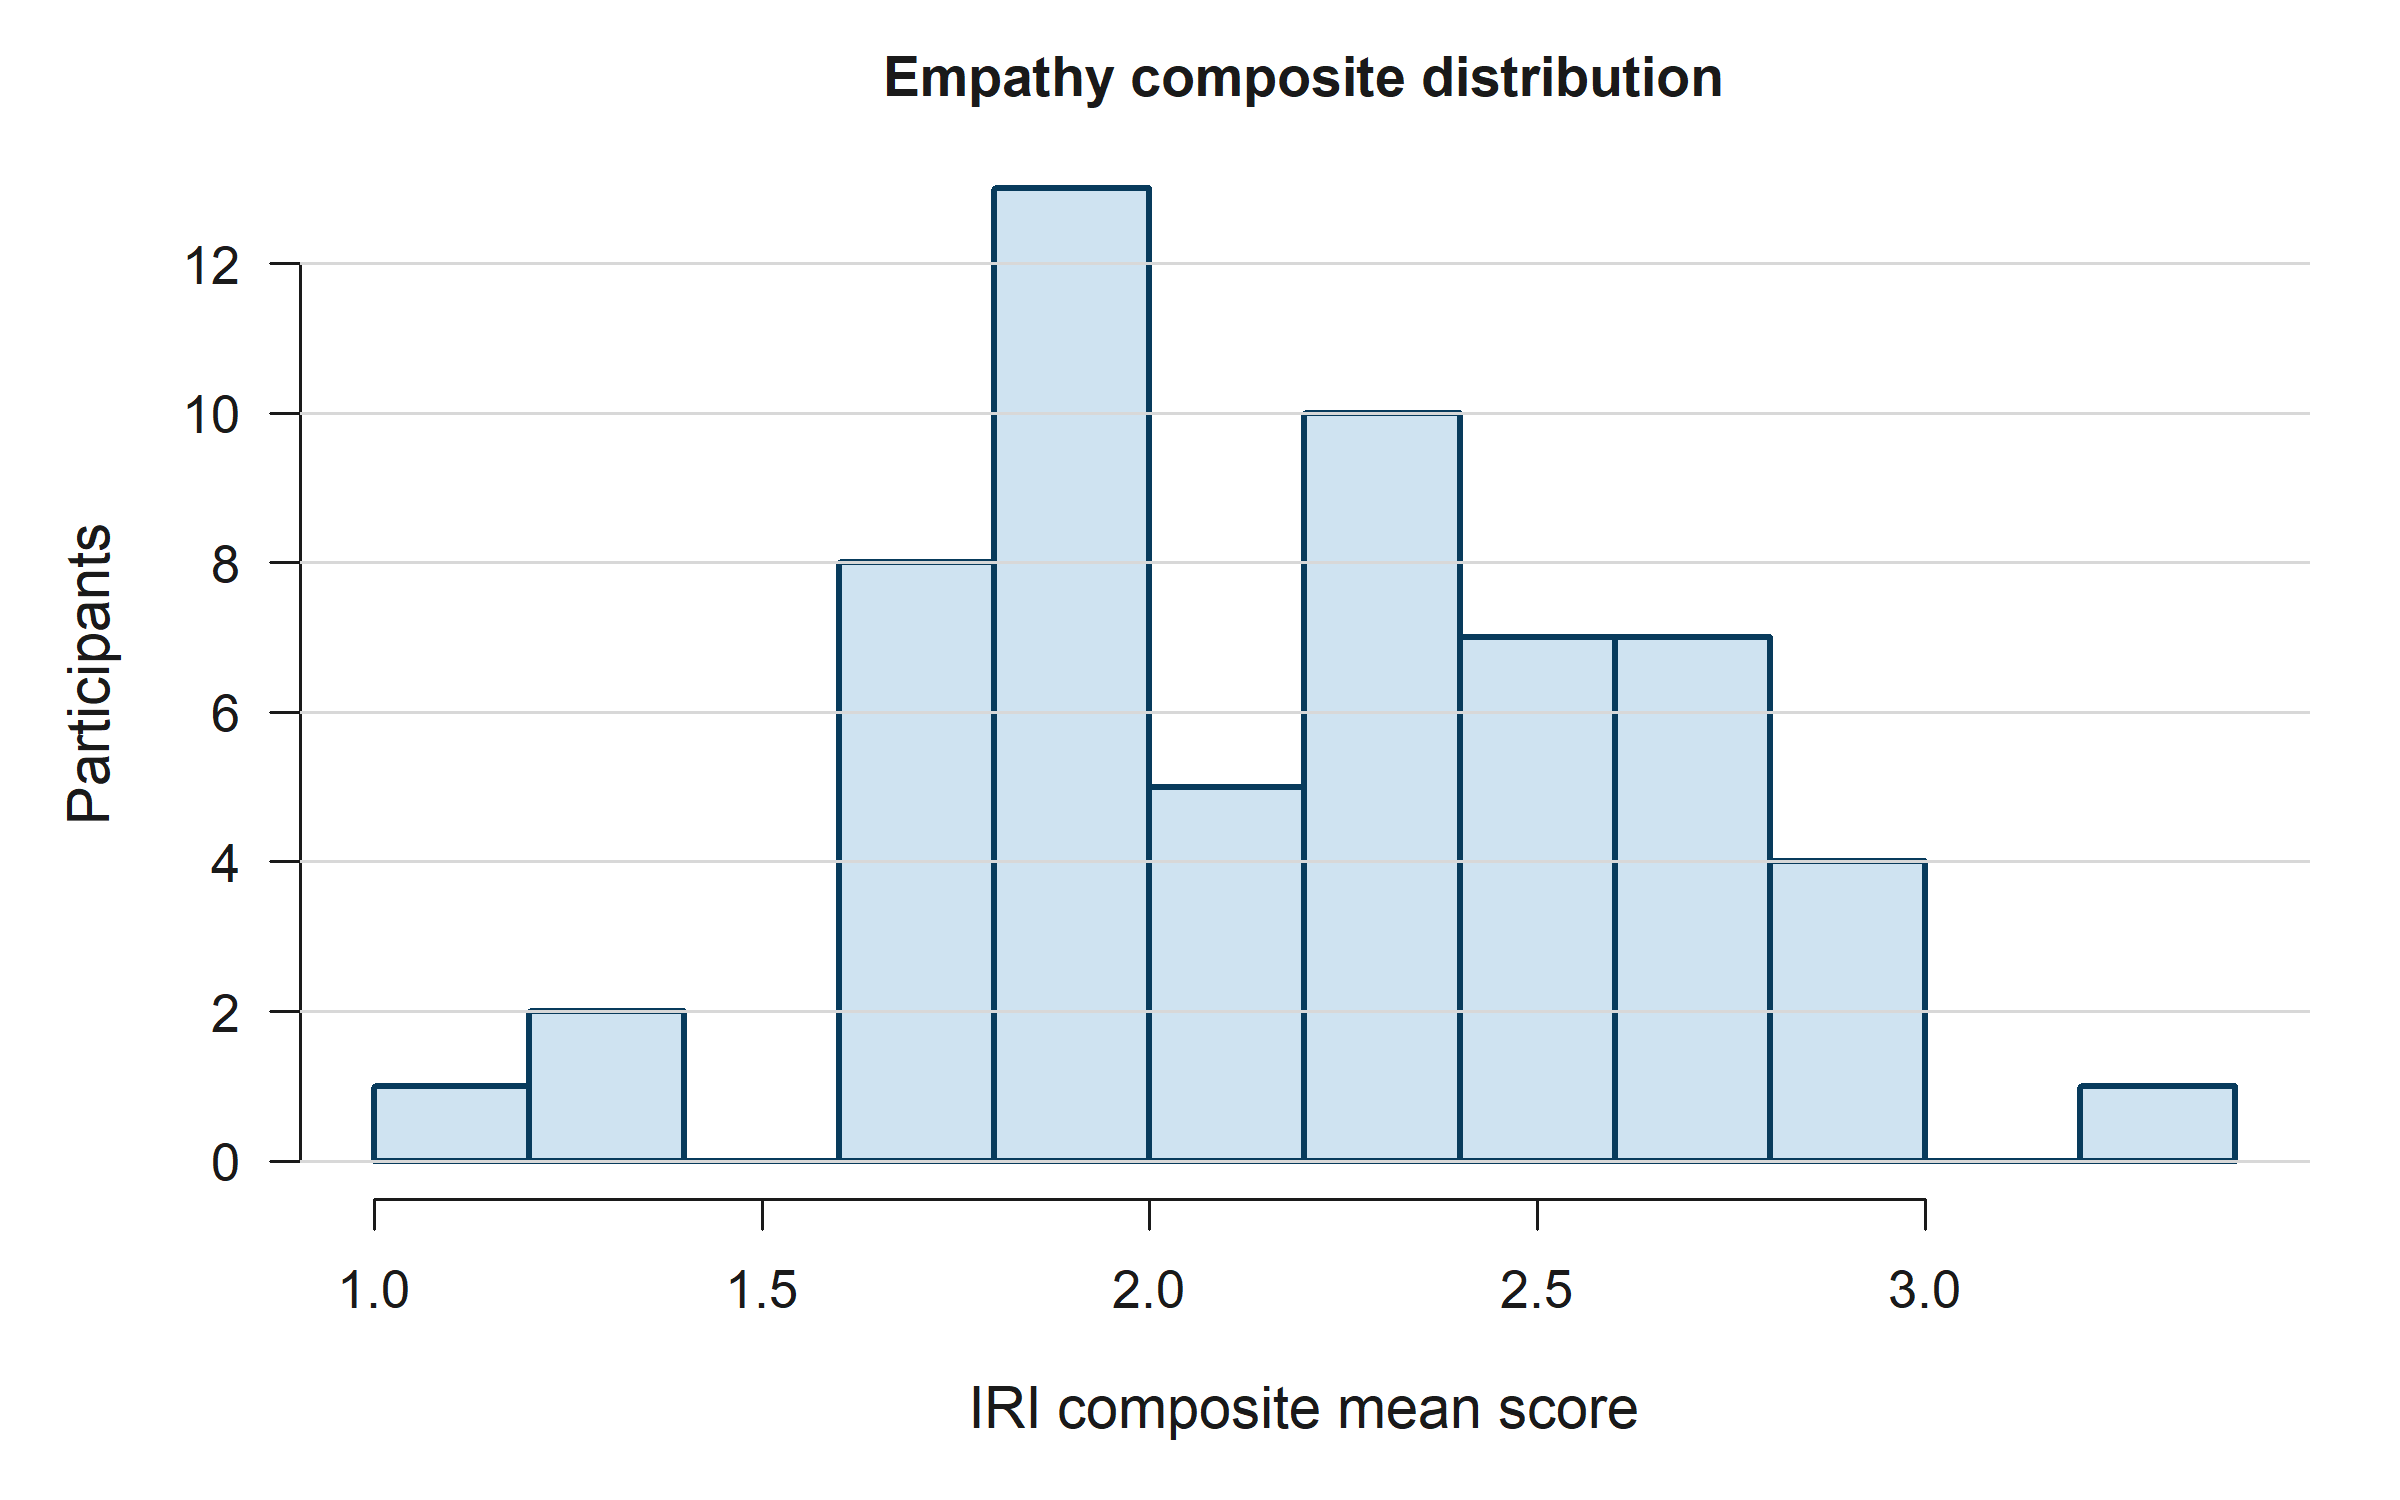
\includegraphics[width=0.92\textwidth]{../figures/figure_02_iri_total_distribution.png}
\caption{Empathy composite distribution.}
\label{fig:empathy}
\end{figure}
\begin{figure}[H]
\centering
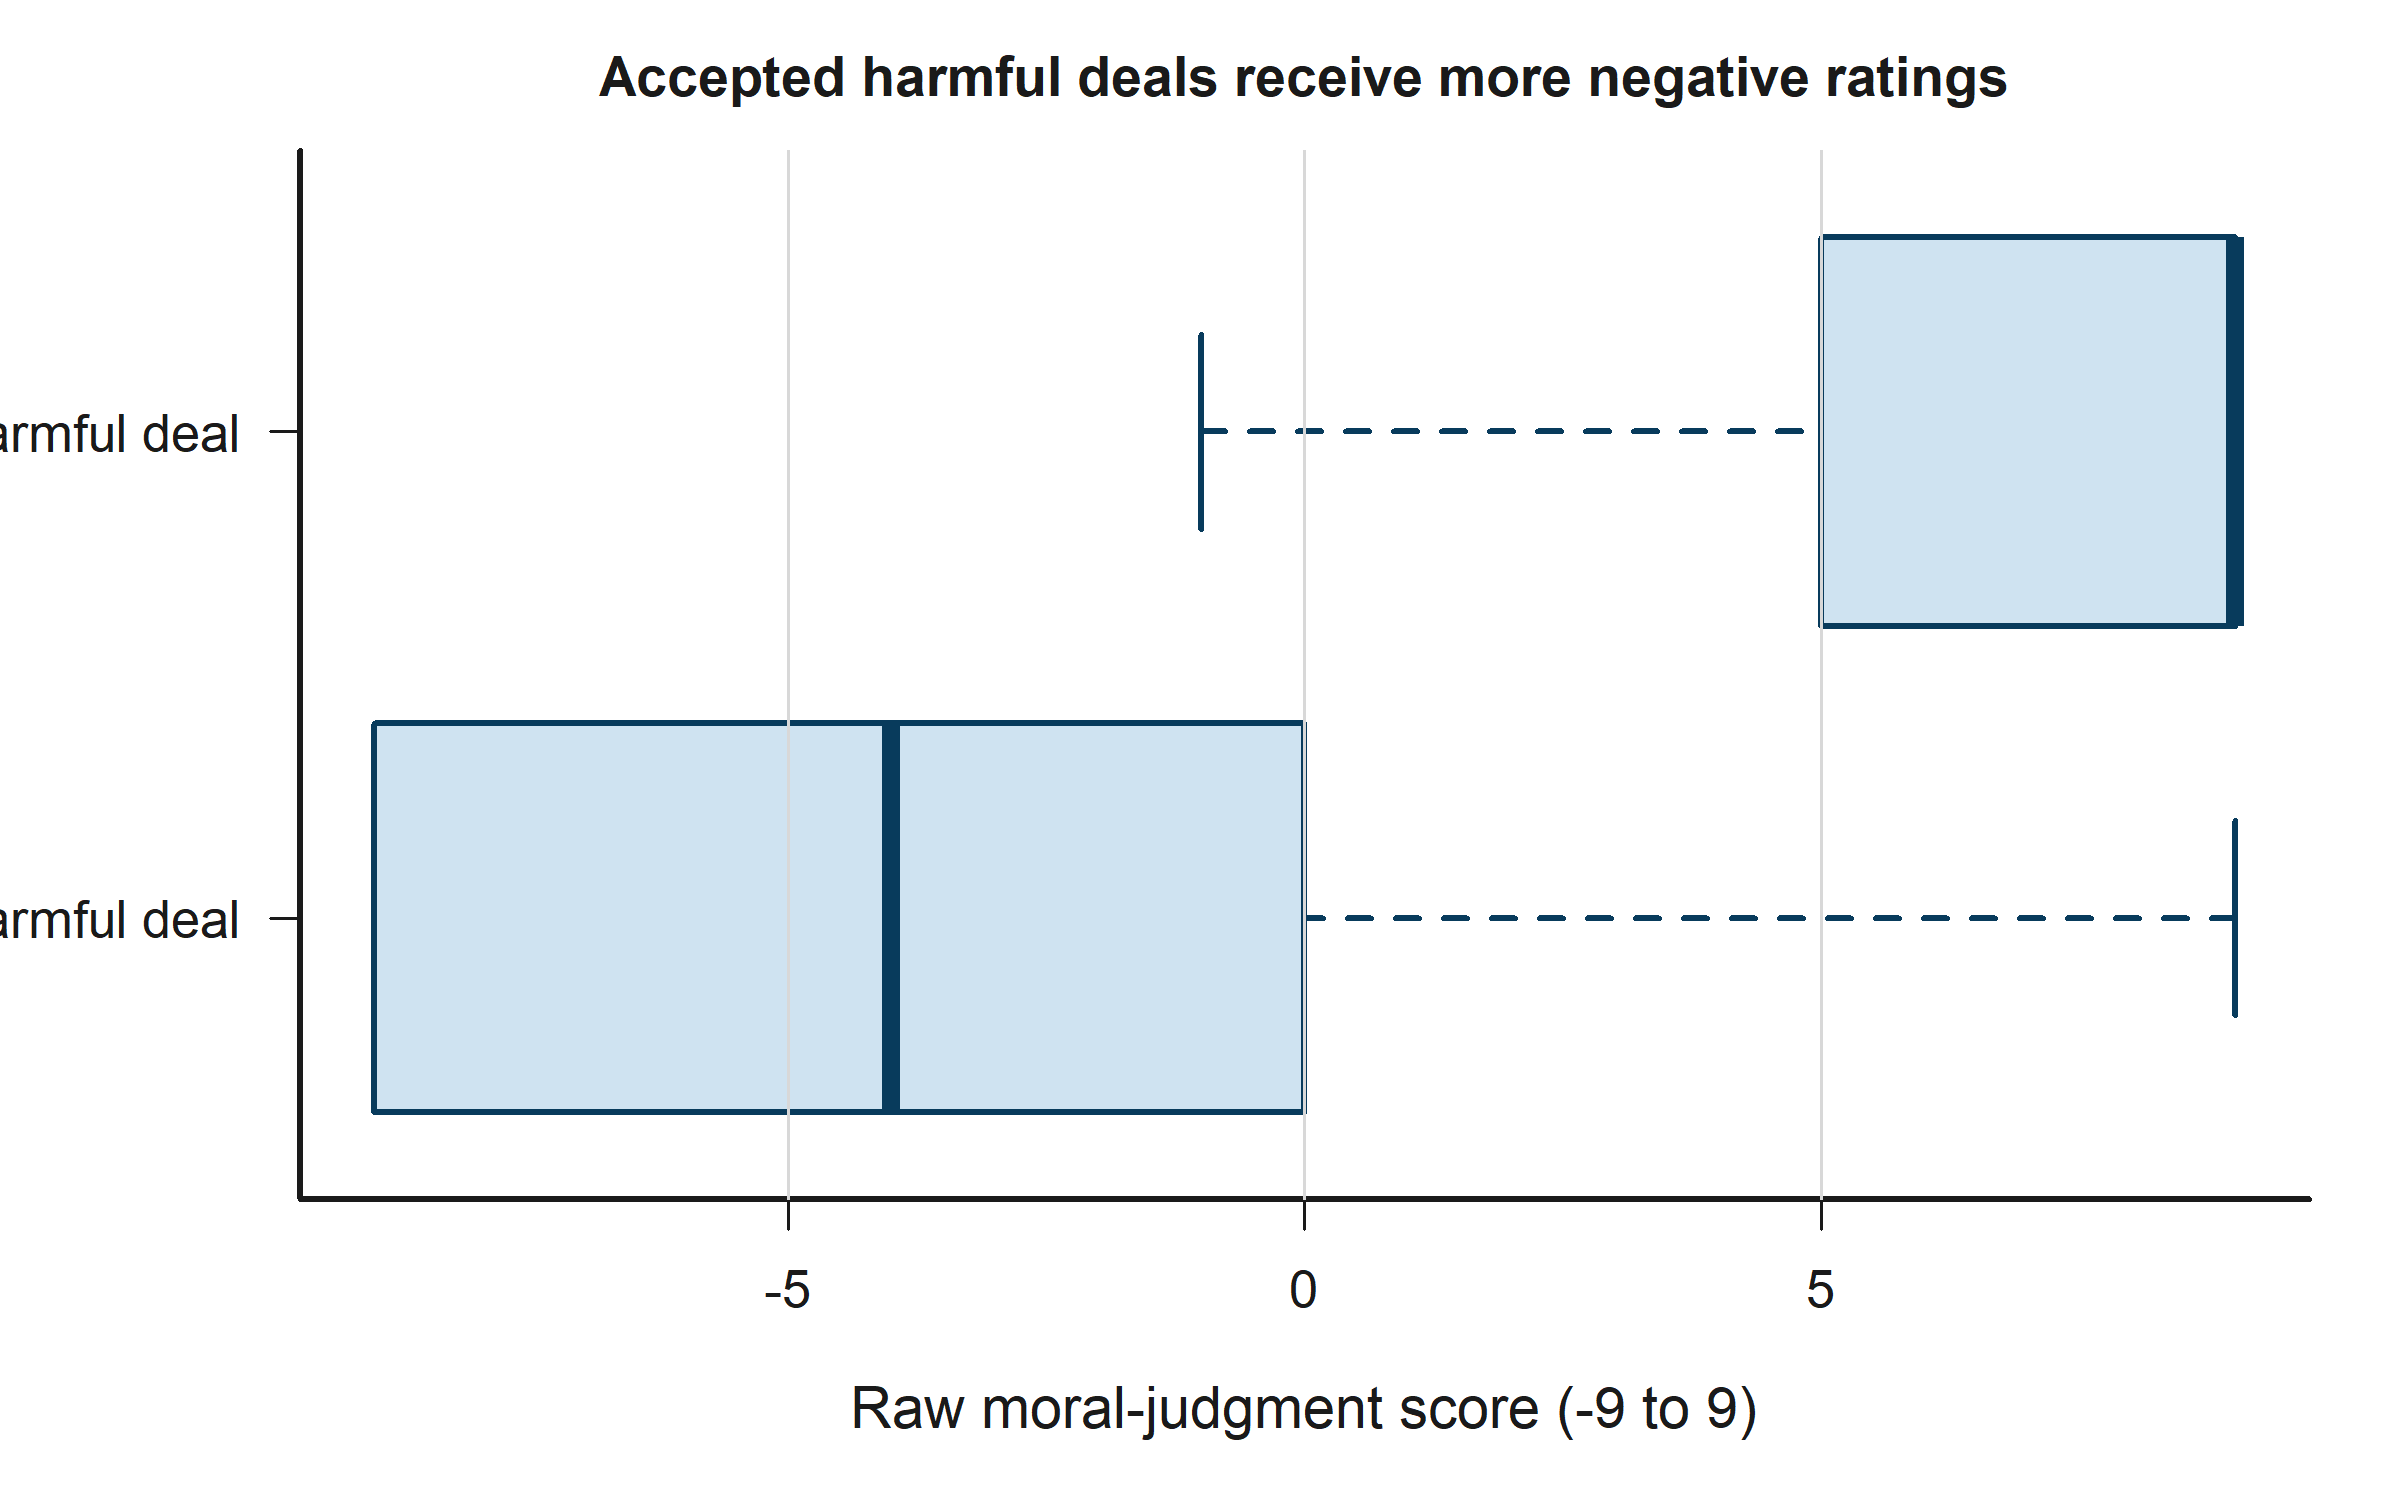
\includegraphics[width=0.92\textwidth]{../figures/figure_03_judgement_by_decision.png}
\caption{Raw moral judgment by decision type.}
\label{fig:decision}
\end{figure}
\begin{figure}[H]
\centering
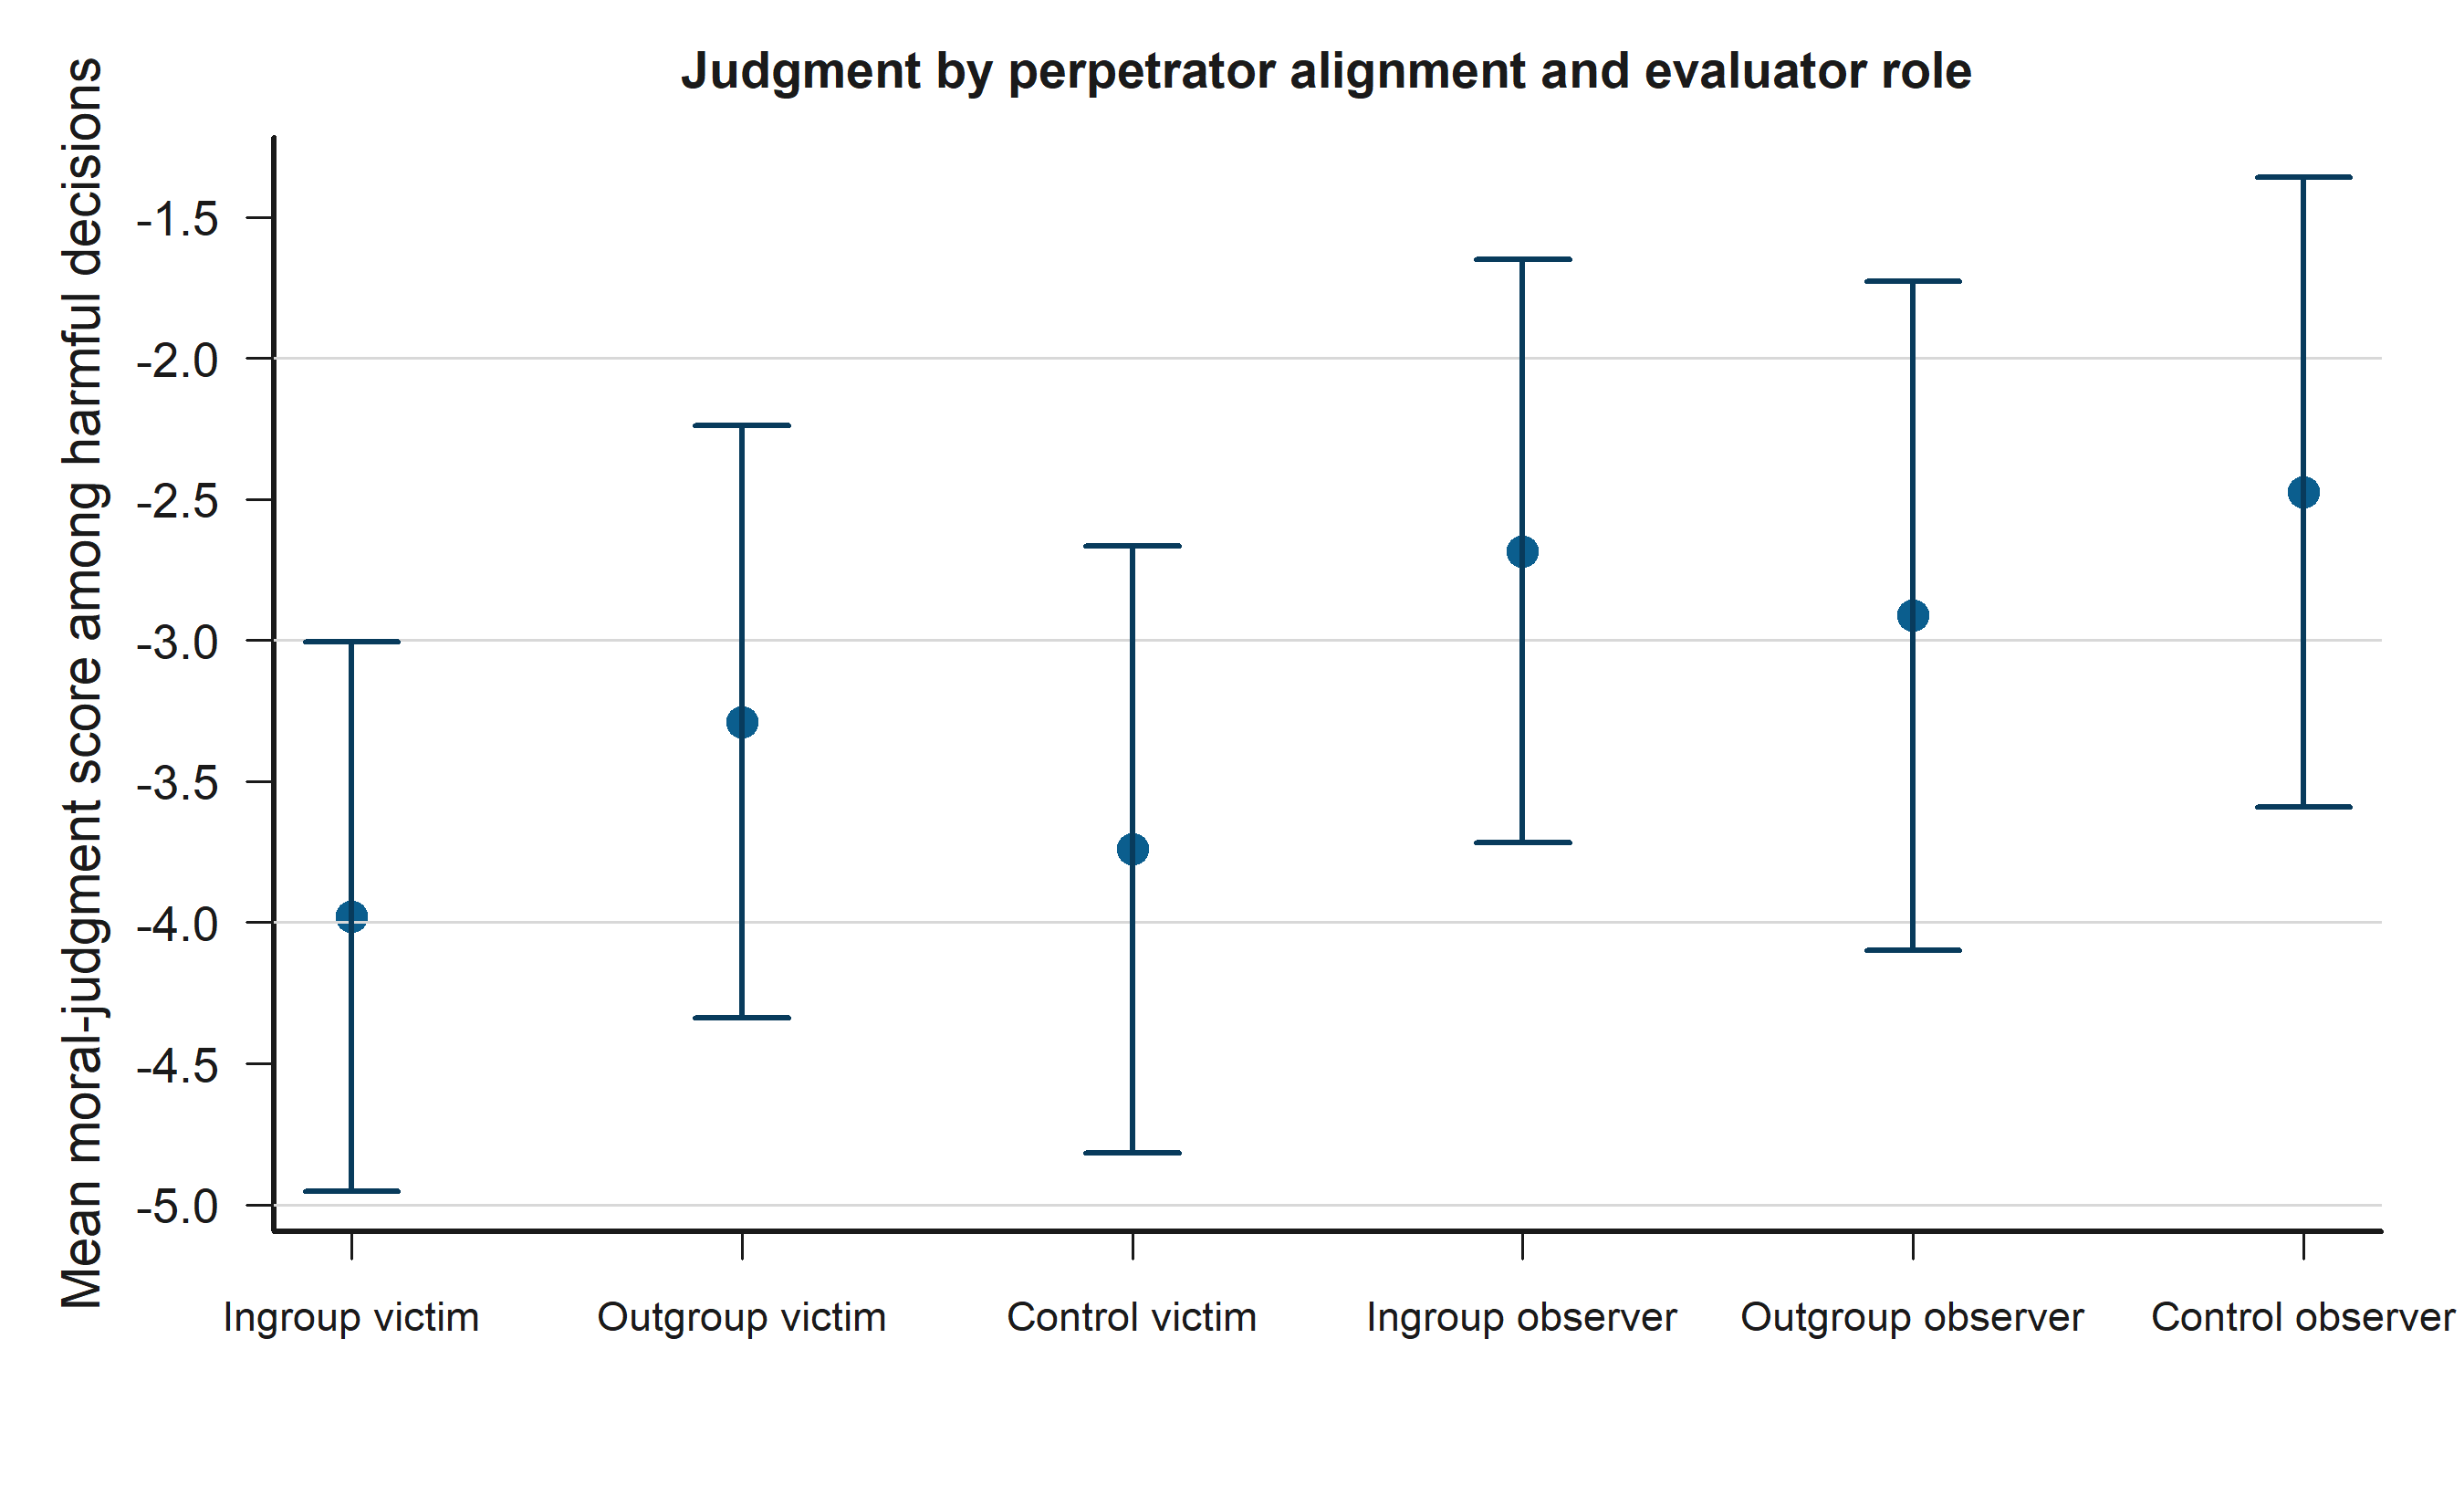
\includegraphics[width=0.92\textwidth]{../figures/figure_04_harmful_decisions_by_group.png}
\caption{Mean judgment by perpetrator alignment and evaluator role.}
\label{fig:group}
\end{figure}
\subsection{Model Results}
In the main harmful-decision Tobit model, higher empathy is associated with harsher judgments (b = -0.79, 95\% CI [-2.86, 1.29], p = 0.457; not statistically distinguishable from zero). Outgroup perpetrators receive more favorable judgments than ingroup perpetrators (b = 0.08, 95\% CI [-1.27, 1.44], p = 0.906; not statistically distinguishable from zero). The empathy slope becomes more negative in outgroup cases than ingroup cases (b = -0.45, 95\% CI [-2.06, 1.16], p = 0.583; not statistically distinguishable from zero). In the same-faculty harm model, same-faculty harm is associated with harsher condemnation (b = -1.34, 95\% CI [-2.88, 0.19], p = 0.087; not statistically distinguishable from zero).
The main harmful-decision Tobit model indicates that empathy has a negative estimated association with judgments, consistent with harsher condemnation at higher empathy, but the estimate is imprecise and not statistically distinguishable from zero (b = -0.79, p = 0.457). The estimated outgroup-perpetrator effect is close to zero and slightly positive (b = 0.08, p = 0.906). The empathy-by-outgroup interaction is negative, which matches the theorized direction for H3, but it is also statistically inconclusive (b = -0.45, p = 0.583). Among the controls, outgroup victims are judged more negatively at the 0.05 threshold and observer-role evaluations are less negative than victim-role evaluations. Across the formal hypothesis tests, all four null hypotheses are retained at alpha = 0.05, although H2a is the closest case to the theorized pattern.
\begin{longtable}{llllll}
\caption{Main harmful-decision Tobit coefficients.}\label{tab:main_tobit}\\
\toprule
Term & Estimate & RobustSE & CI\_Low & CI\_High & PValue \\
\midrule
\endfirsthead
\toprule
Term & Estimate & RobustSE & CI\_Low & CI\_High & PValue \\
\midrule
\endhead
Intercept & 0.508 & 5.090 & -9.468 & 10.484 & 0.921 \\
Empathy composite (z) & -0.788 & 1.059 & -2.864 & 1.288 & 0.457 \\
Outgroup perpetrator (ref = ingroup) & 0.082 & 0.691 & -1.272 & 1.436 & 0.906 \\
Control label hidden (ref = ingroup) & 0.139 & 0.807 & -1.443 & 1.721 & 0.863 \\
Victim outgroup (ref = ingroup) & -2.417 & 1.233 & -4.834 & -0.000 & 0.050 \\
Observer role (ref = victim) & 2.890 & 1.394 & 0.158 & 5.622 & 0.038 \\
Engineering participant (ref = humanities) & -1.279 & 1.801 & -4.808 & 2.251 & 0.478 \\
Man (ref = woman) & -1.821 & 1.761 & -5.273 & 1.631 & 0.301 \\
Age & -0.089 & 0.218 & -0.516 & 0.338 & 0.683 \\
Socioeconomic status & -0.435 & 0.760 & -1.923 & 1.054 & 0.567 \\
Stage 2 (ref = stage 1) & 0.769 & 1.056 & -1.301 & 2.840 & 0.466 \\
Stage 3 (ref = stage 1) & -1.132 & 1.450 & -3.973 & 1.710 & 0.435 \\
Stage 4 (ref = stage 1) & -2.214 & 1.528 & -5.208 & 0.781 & 0.147 \\
Stage 5 (ref = stage 1) & -1.788 & 1.250 & -4.238 & 0.662 & 0.153 \\
Stage 6 (ref = stage 1) & -0.749 & 1.348 & -3.391 & 1.893 & 0.578 \\
Stage 7 (ref = stage 1) & -1.454 & 1.237 & -3.878 & 0.970 & 0.240 \\
Stage 8 (ref = stage 1) & -3.178 & 1.407 & -5.936 & -0.421 & 0.024 \\
Stage 9 (ref = stage 1) & -2.733 & 1.358 & -5.394 & -0.071 & 0.044 \\
Stage 10 (ref = stage 1) & -1.122 & 1.359 & -3.787 & 1.542 & 0.409 \\
Negotiator 2 (ref = negotiator 1) & 0.002 & 0.485 & -0.948 & 0.953 & 0.996 \\
Empathy x outgroup perpetrator & -0.450 & 0.821 & -2.059 & 1.159 & 0.583 \\
Empathy x control label hidden & -0.450 & 0.733 & -1.887 & 0.987 & 0.539 \\
\bottomrule
\end{longtable}
\begin{longtable}{llllll}
\caption{Same-group-harm Tobit coefficients.}\label{tab:betrayal_tobit}\\
\toprule
Term & Estimate & RobustSE & CI\_Low & CI\_High & PValue \\
\midrule
\endfirsthead
\toprule
Term & Estimate & RobustSE & CI\_Low & CI\_High & PValue \\
\midrule
\endhead
Intercept & 4.054 & 5.531 & -6.788 & 14.895 & 0.464 \\
Empathy composite (z) & -0.873 & 0.953 & -2.740 & 0.994 & 0.359 \\
Negotiator and victim share faculty & -1.341 & 0.783 & -2.876 & 0.194 & 0.087 \\
Outgroup perpetrator (ref = ingroup) & -0.578 & 0.721 & -1.991 & 0.835 & 0.423 \\
Victim outgroup (ref = ingroup) & -1.847 & 1.534 & -4.854 & 1.160 & 0.229 \\
Observer role (ref = victim) & 2.294 & 1.520 & -0.685 & 5.272 & 0.131 \\
Engineering participant (ref = humanities) & -1.755 & 1.764 & -5.211 & 1.702 & 0.320 \\
Man (ref = woman) & -1.175 & 1.774 & -4.652 & 2.302 & 0.508 \\
Age & -0.213 & 0.227 & -0.659 & 0.233 & 0.349 \\
Socioeconomic status & -0.303 & 0.735 & -1.743 & 1.137 & 0.680 \\
Stage 2 (ref = stage 1) & -0.630 & 1.527 & -3.623 & 2.363 & 0.680 \\
Stage 3 (ref = stage 1) & -0.843 & 1.536 & -3.855 & 2.168 & 0.583 \\
Stage 4 (ref = stage 1) & -3.761 & 1.511 & -6.722 & -0.800 & 0.013 \\
Stage 5 (ref = stage 1) & -1.283 & 1.822 & -4.853 & 2.288 & 0.481 \\
Stage 6 (ref = stage 1) & -0.760 & 1.393 & -3.490 & 1.970 & 0.585 \\
Stage 7 (ref = stage 1) & -2.578 & 1.478 & -5.475 & 0.319 & 0.081 \\
Stage 8 (ref = stage 1) & -2.125 & 1.470 & -5.005 & 0.756 & 0.148 \\
Stage 9 (ref = stage 1) & -1.470 & 1.362 & -4.139 & 1.199 & 0.280 \\
Stage 10 (ref = stage 1) & -1.463 & 1.611 & -4.622 & 1.695 & 0.364 \\
Negotiator 2 (ref = negotiator 1) & -0.147 & 0.576 & -1.277 & 0.982 & 0.798 \\
\bottomrule
\end{longtable}
\begin{table}[H]
\centering
\caption{Model fit summary.}
\label{tab:model_fit}
\begin{tabular}{llllllll}
\toprule
Model & Observations & Participants & LowerBoundCensored & UpperBoundCensored & LogLik & AIC & PseudoR2 \\
\midrule
Main harmful-decision Tobit & 569 & 58 & 170 & 27 & -1458.903 & 2963.805 & 0.014 \\
Same-faculty harm Tobit & 364 & 58 & 103 & 13 & -941.867 & 1925.733 & 0.013 \\
Full-sample Tobit & 1160 & 58 & 182 & 332 & -2627.999 & 5303.998 & 0.117 \\
\bottomrule
\end{tabular}
\end{table}
\subsection{Hypothesis Tests and Decisions}
Decision rule: reject H0 when p < 0.05; otherwise fail to reject H0. Support for the research hypothesis requires both statistical detectability and the theorized sign.
H1: Fail to reject H0; Insufficient evidence for HA. H1 is inconclusive: fail to reject the null. The coefficient direction is negative but the estimate is not statistically distinguishable from zero. H2a: Fail to reject H0; Insufficient evidence for HA. H2a is inconclusive: fail to reject the null. The coefficient direction is negative but the estimate is not statistically distinguishable from zero. H2b: Fail to reject H0; Insufficient evidence for HA. H2b is inconclusive: fail to reject the null. The coefficient direction is positive but the estimate is not statistically distinguishable from zero. H3: Fail to reject H0; Insufficient evidence for HA. H3 is inconclusive: fail to reject the null. The coefficient direction is negative but the estimate is not statistically distinguishable from zero.
\begin{longtable}{llllllllll}
\caption{Hypothesis validation table.}\label{tab:hypothesis_validation}\\
\toprule
Hypothesis & Description & ModelTerm & Estimate & CI95 & PValue & Verdict & NullDecision & ResearchDecision & Interpretation \\
\midrule
\endfirsthead
\toprule
Hypothesis & Description & ModelTerm & Estimate & CI95 & PValue & Verdict & NullDecision & ResearchDecision & Interpretation \\
\midrule
\endhead
H1 & Higher empathy predicts lower moral-judgment scores for harmful decisions. & Empathy composite (z) & -0.788 & [-2.86, 1.29] & 0.457 & Inconclusive & Fail to reject H0 & Insufficient evidence for HA & H1 is inconclusive: fail to reject the null. The coefficient direction is negative but the estimate is not statistically distinguishable from zero. \\
H2a & Same-faculty harm receives lower moral-judgment scores than cross-faculty harm. & Negotiator and victim share faculty & -1.341 & [-2.88, 0.19] & 0.087 & Inconclusive & Fail to reject H0 & Insufficient evidence for HA & H2a is inconclusive: fail to reject the null. The coefficient direction is negative but the estimate is not statistically distinguishable from zero. \\
H2b & Outgroup perpetrators receive lower moral-judgment scores than ingroup perpetrators. & Outgroup perpetrator (ref = ingroup) & 0.082 & [-1.27, 1.44] & 0.906 & Inconclusive & Fail to reject H0 & Insufficient evidence for HA & H2b is inconclusive: fail to reject the null. The coefficient direction is positive but the estimate is not statistically distinguishable from zero. \\
H3 & Empathy becomes more negative in outgroup than ingroup cases. & Empathy x outgroup perpetrator & -0.450 & [-2.06, 1.16] & 0.583 & Inconclusive & Fail to reject H0 & Insufficient evidence for HA & H3 is inconclusive: fail to reject the null. The coefficient direction is negative but the estimate is not statistically distinguishable from zero. \\
\bottomrule
\end{longtable}
\section{Assumptions}
The Tobit model is appropriate here because the observed dependent variable is bounded at -9 and 9 and the sample includes observations piled up at both limits. In the harmful-decision sample there are 569 negotiator-level observations from 58 participants. The observed censoring shares are 29.9\% at the lower bound and 4.7\% at the upper bound. Substantive interpretation assumes a latent continuous evaluation process, approximately normal model errors, and correct specification of the linear predictor. Inference is clustered by participant to address repeated judgments within persons, but the estimates should still be read cautiously because the participant count is modest.
\section{Discussion}
The results suggest that the study has some directional consistency with the empathy and ingroup-betrayal accounts, but the evidence is not strong enough to support the research hypotheses under a conventional 5 percent threshold. The clearest substantive pattern is the negative point estimate for same-group harm, which is compatible with ingroup betrayal, yet still too uncertain for a firm conclusion (p = 0.087). The lack of support for H2b indicates little evidence that outgroup perpetrators are condemned more harshly in this sample. Given the modest number of participants, repeated judgments nested within persons, and substantial censoring at the lower bound, the null findings should be interpreted as limited evidence rather than strong evidence of no effect.
\section{Conclusions}
In conclusion, the bounded moral-judgment data are well suited to a Tobit framework, and the reporting pipeline now documents the full workflow from raw workbook to publication-style outputs. On the current data, the estimated effects do not justify rejecting the null hypotheses for H1, H2a, H2b, or H3 at alpha = 0.05. The most promising signal is the negative same-group-harm coefficient, which may warrant follow-up with a larger sample or a design with stronger identity contrasts.
\section{Reproducibility Notes}
The pipeline exports synchronized outputs in CSV, PNG, Markdown, Word, LaTeX, and PDF formats. The LaTeX and PDF outputs are generated directly from the fitted model results in the same run as the other reports.
\end{document}
